%% Copyright (C) 2009-2011, Gostai S.A.S.
%%
%% This software is provided "as is" without warranty of any kind,
%% either expressed or implied, including but not limited to the
%% implied warranties of fitness for a particular purpose.
%%
%% See the LICENSE file for more information.

\chapter{Introduction}

\usdk is a fully-featured environment to orchestrate complex
organizations of components.  It relies on a middleware architecture
that coordinates components named UObjects.  It also features \us, a
scripting language that can be used to write orchestration programs.

\section{\urbi and UObjects}

\urbi makes the orchestration of independent, concurrent, components easier.
It was first designed for robotics: it provides all the needed features to
coordinate the execution of various components (actuators, sensors, software
devices that provide features such as text-to-speech, face recognition and
so forth).  Languages such as \Cxx are well suited to program the local,
low-level, handling of these hardware or software devices; indeed one needs
efficiency, small memory footprint, and access to low-level hardware
details.  Yet, when it comes to component orchestration and coordination, in
a word, when it comes to addressing concurrency, it can be tedious to use
such languages.

Middleware infrastructures make possible to use remote components as if they
were local, to allow concurrent execution, to make synchronous or
asynchronous requests and so forth.  The \dfn{UObject} \Cxx architecture
provides exactly this: a common API that allows conforming components to be
used seamlessly in highly concurrent settings.  Components need not be
designed with UObjects in mind, rather, UObjects are typically ``shells''
around ``regular'' components.

Components with an UObject interface are naturally supported by the \us
programming language.  This provides a tremendous help: one can interact
with these components (making queries, changing them, observing their state,
monitoring various kinds of events and so forth), which provides a huge
speed-up during development.

Although made with robots in mind, the UObject architecture is well suited
to tame any heavily concurrent environment, such as video games or complex
systems in general.

\section{The Big Picture}

The \autoref{fig:arch} shows the architecture of \urbi.  Let's browse it
bottom up.

\begin{figure}[p]
  \centering
  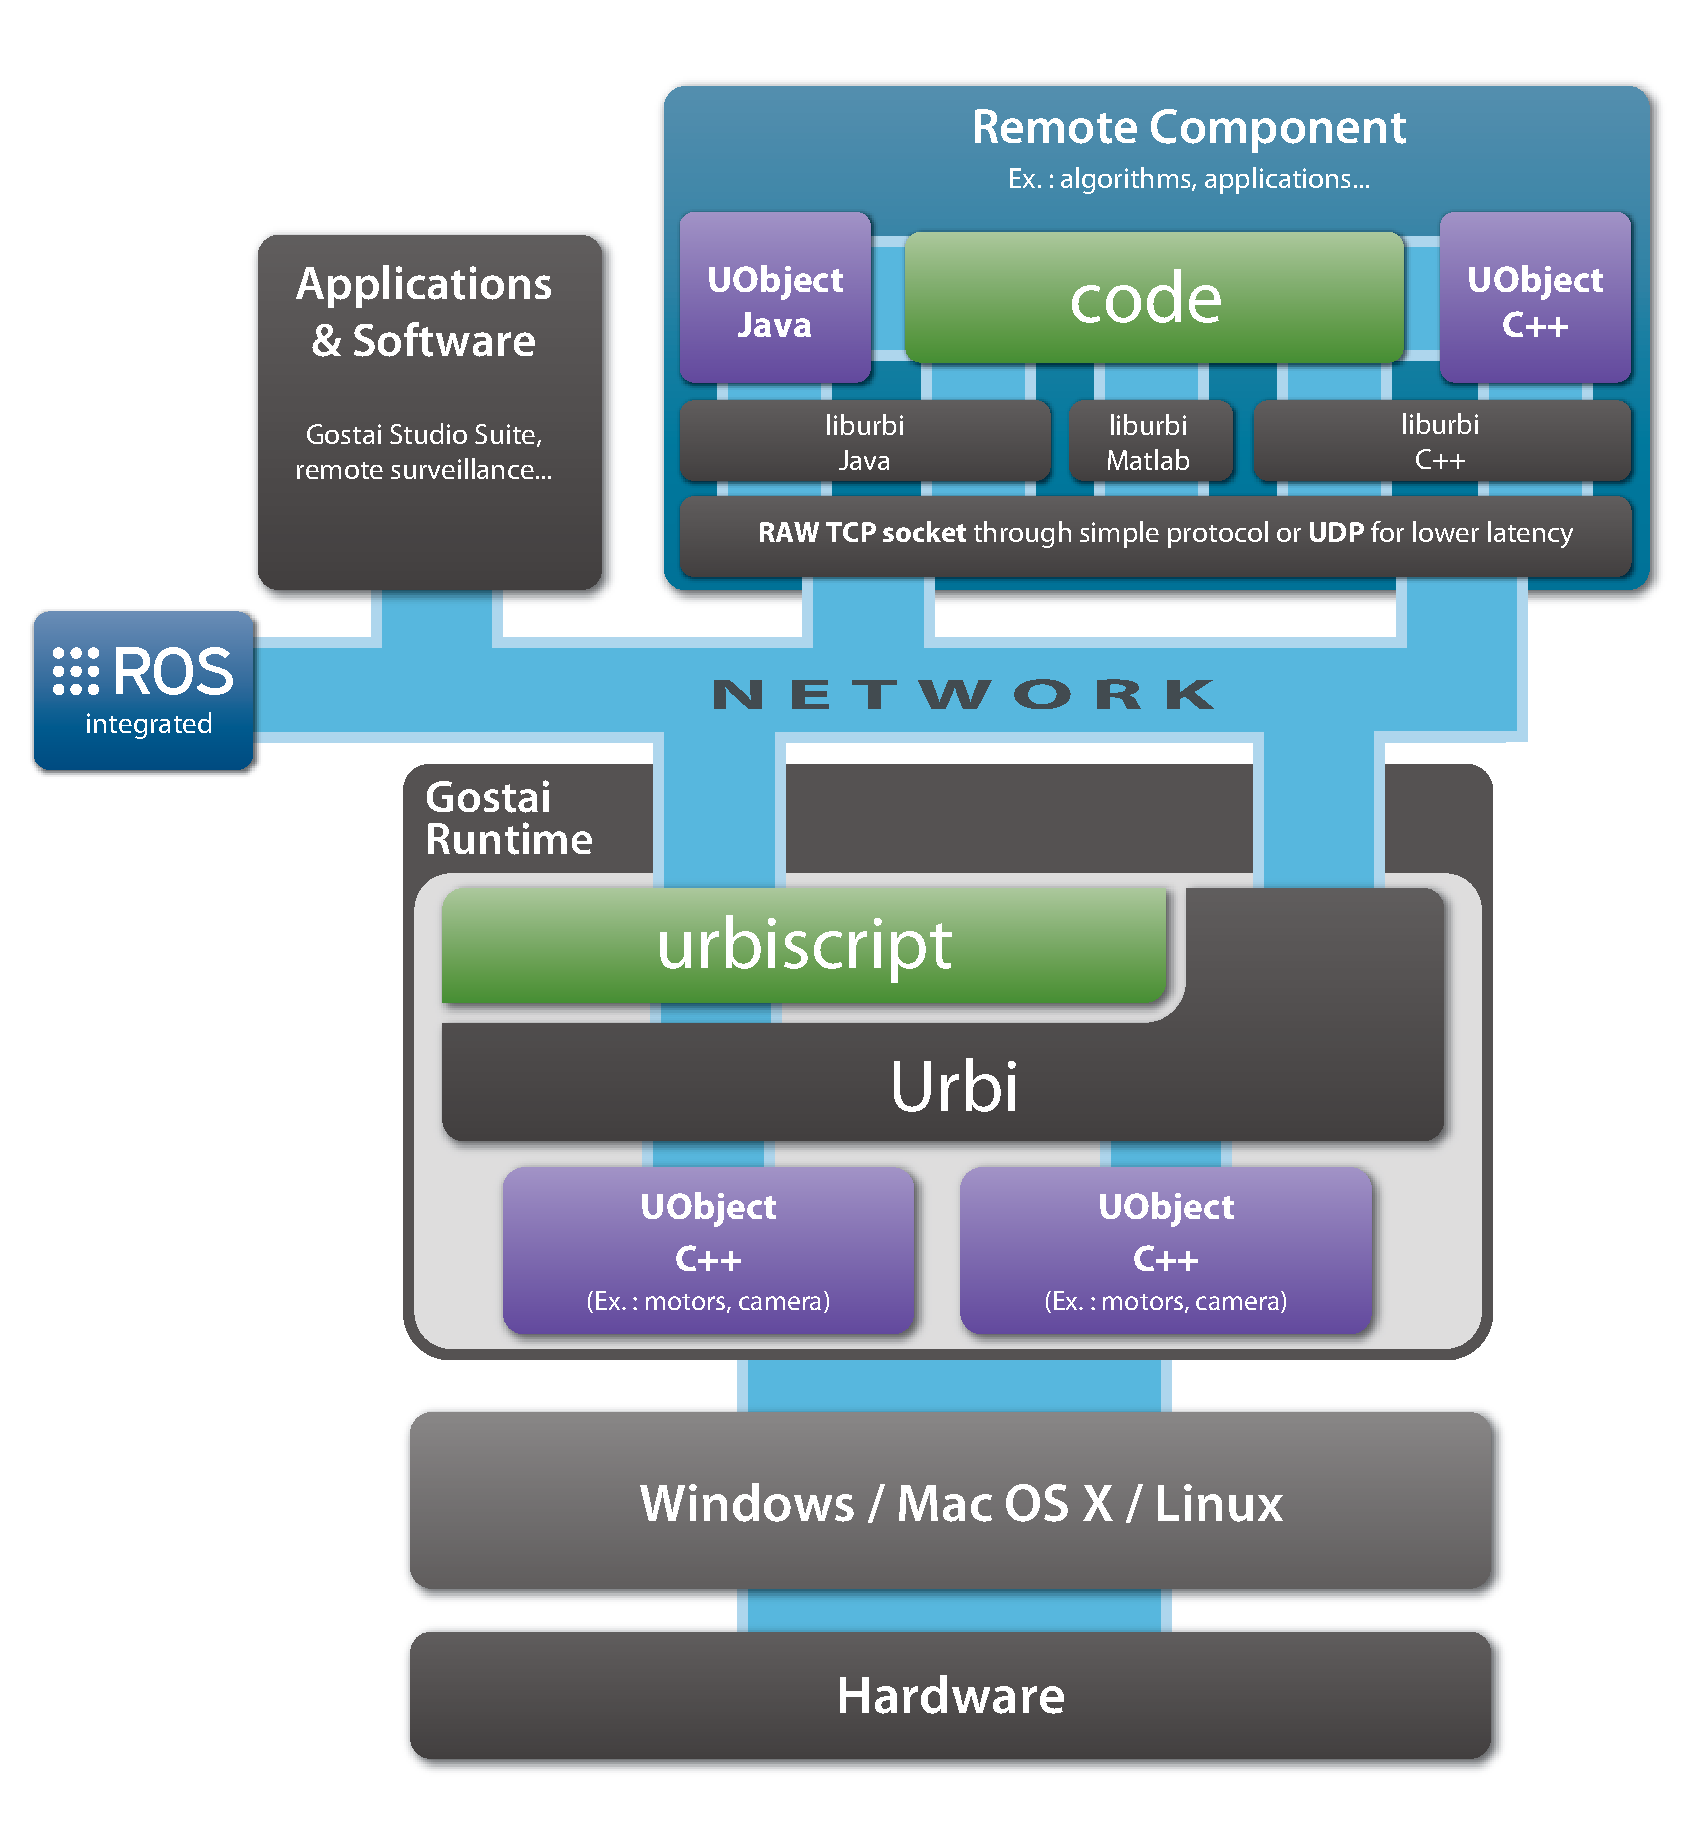
\includegraphics[width=\linewidth]{img/urbi-architecture}
  \caption{A Bird-View of the \urbi Architecture}
  \label{fig:arch}
\end{figure}

At the lowest level, \urbi requires a (possibly very limited) embedded
computer.  This is the case for most robots today, but on occasion, some
device cannot even run reasonably small pieces of code.  In that case, \urbi
can still be used, but then the robot is actually remote-controlled from a
computer running \urbi.

Right on top of the hardware, is running the \dfn{Operating System}.  \urbi
supports the major OSes; it was also ported on top of real-time OSes such as
Xenomai, and on specific OSes such as Aperios, Sony's proprietary system
running its Aibo robotic dog.

The \dfn{Urbi Runtime}, which is the actual core of the system, also known
as the \dfn{engine} or the \dfn{kernel}, is interfacing the OS with the rest
of the \urbi world, \us and UObjects.

UObjects are used to bind hardware or software components, such as
actuators and sensors on the one hand, and voice synthesis or face
recognition on the other hand.  They can be run locally on the robot, or on
a remote, more powerful, computer.

To orchestrate all the components, \us is a programming language of choice
(see below).

Finally, applications are available for the \urbi environment.  For
instance, Gostai Studio provides high-level tools to develop complex robotic
behaviors.

\section{\urbi and \us}

\us is a programming language primarily designed for robotics. It's a
dynamic, prototype-based, object-oriented scripting language. It supports
and emphasizes parallel and event-based programming, which are very popular
paradigms in robotics, by providing core primitives and language constructs.

\medskip

Its main features are:
\begin{itemize}
\item syntactically close to \Cxx.\\
  If you know \C, \Cxx, \Java, or JavaScript, you can easily write \us
  programs.
\item fully integrated with \Cxx.\\
  You can bind \Cxx classes in \us seamlessly. \us is also integrated with
  many other languages such as \Java, \MatLab or \Python.
\item object-oriented.\\
  It supports encapsulation, inheritance and inclusion polymorphism. Dynamic
  dispatching is available through monomethods --- just as \Cxx, \Cs or
  \Java.
\item concurrent.\\
  It provides you with natural constructs to run and control high numbers of
  interacting concurrent tasks.
\item event-based.\\
  Triggering events and reacting to them is absolutely straightforward.
\item functional programming.\\
  Inspired by languages such as \Lisp or \Caml, \us features first class
  functions and pattern matching.
\item client/server.\\
  The interpreter accepts multiple connections from different sources (human
  users, robots, other servers \ldots) and enables them to interact.
\item distributed.\\
  You can run objects in different processes, potentially remote computers
  across the network.
\end{itemize}

\section{Genesis}

\urbi what first designed and implemented by Jean-Christophe Baillie,
together with Matthieu Nottale.  Because its users wildly acclaimed it,
Jean-Christophe founded Gostai, a France-based Company that develops
software for robotics with a strong emphasis on personal robotics.

\paragraph{Authors}
\usdk 1 was further developed by Akim Demaille, Guillaume Deslandes, Quentin
Hocquet, and Benoît Sigoure.

The \usdk 2 project was started and developed by Akim Demaille, Quentin
Hocquet, Matthieu Nottale, and Benoît Sigoure.  Samuel Tardieu provided an
immense help during the year 2008, in particular for the concurrency and
event support.

The maintenance is currently carried out by Akim Demaille, Quentin
Hocquet, and Matthieu Nottale.  Jean-Christophe Baillie is still
deeply involved in the development of \us, he regularly submits ideas,
and occasionally even code!

\paragraph{Contributors}

A number of people contributed significantly to \urbi, including Alexandre
Morgand, Romain Bezut, Thomas Moulard, Clément Moussu, Nicolas Pierron.

\section{Outline}

This multi-part document provides a complete guide to Urbi.  See
\autoref{sec:notations} for the various notations that are used in the
document.

\newenvironment{partDescription}[2]
{%
  \item[\autoref{#1} --- \nameref{#1}]~\\%
  #2
  \begin{description}%
    \let\itemOrig\item%
    \renewcommand{\item}[1][]{\itemOrig[~~\autoref{##1} --- \nameref{##1}]~\\}%
  }{%
  \end{description}%
}

%%% Keep sync with urbi-sdk.tex.
\begin{description}
%% Copyright (C) 2010, Gostai S.A.S.
%%
%% This software is provided "as is" without warranty of any kind,
%% either expressed or implied, including but not limited to the
%% implied warranties of fitness for a particular purpose.
%%
%% See the LICENSE file for more information.

\begin{partDescription}{part:tut}
  {%
    This part, also known as the ``\us tutorial'', teaches the reader
    how to program in
    \us.  It goes from the basis to concurrent and
    event-based programming.  No specific knowledge is expected.
    There is no need for a \Cxx compiler, as \UObject will not be
    covered here (see \autoref{part:uobject}).  The reference manual
    contains a terse and complete definition of the \urbi environment
    (\autoref{part:specs}).
    %
  }
\item[sec:tut:first]
  First contacts with \us.
\item[sec:tut:value]
  A quick introduction to objects and values.
\item[sec:tut:flow]
  Basic control flow: \lstinline{if}, \lstinline{for} and the like.
\item[sec:tut:function]
  Details about functions, scoped, and lexical closures.
\item[sec:tut:object]
  A more in-depth introduction to object-oriented programming in \us.
\item[sec:tut:functional]
  Functions are first-class citizens.
\item[sec:tut:concurrent]
  The \us operators for concurrency, tags.
\item[sec:tut:event-prog]
  Support for event-driven concurrency in \us.
\item[sec:tut:ros] How to use ROS from \urbi, and vice-versa.
\end{partDescription}


%%% Local Variables:
%%% mode: latex
%%% TeX-master: "../urbi-sdk"
%%% ispell-dictionary: "american"
%%% ispell-personal-dictionary: "../urbi.dict"
%%% fill-column: 76
%%% End:

%% Copyright (C) 2010, Gostai S.A.S.
%%
%% This software is provided "as is" without warranty of any kind,
%% either expressed or implied, including but not limited to the
%% implied warranties of fitness for a particular purpose.
%%
%% See the LICENSE file for more information.

\begin{partDescription}{part:tut}
  {%
    This part, also known as the ``\us tutorial'', teaches the reader
    how to program in
    \us.  It goes from the basis to concurrent and
    event-based programming.  No specific knowledge is expected.
    There is no need for a \Cxx compiler, as \UObject will not be
    covered here (see \autoref{part:uobject}).  The reference manual
    contains a terse and complete definition of the \urbi environment
    (\autoref{part:specs}).
    %
  }
\item[sec:tut:first]
  First contacts with \us.
\item[sec:tut:value]
  A quick introduction to objects and values.
\item[sec:tut:flow]
  Basic control flow: \lstinline{if}, \lstinline{for} and the like.
\item[sec:tut:function]
  Details about functions, scoped, and lexical closures.
\item[sec:tut:object]
  A more in-depth introduction to object-oriented programming in \us.
\item[sec:tut:functional]
  Functions are first-class citizens.
\item[sec:tut:concurrent]
  The \us operators for concurrency, tags.
\item[sec:tut:event-prog]
  Support for event-driven concurrency in \us.
\item[sec:tut:ros] How to use ROS from \urbi, and vice-versa.
\end{partDescription}


%%% Local Variables:
%%% mode: latex
%%% TeX-master: "../urbi-sdk"
%%% ispell-dictionary: "american"
%%% ispell-personal-dictionary: "../urbi.dict"
%%% fill-column: 76
%%% End:

%% Copyright (C) 2010, Gostai S.A.S.
%%
%% This software is provided "as is" without warranty of any kind,
%% either expressed or implied, including but not limited to the
%% implied warranties of fitness for a particular purpose.
%%
%% See the LICENSE file for more information.

\begin{partDescription}{part:tut}
  {%
    This part, also known as the ``\us tutorial'', teaches the reader
    how to program in
    \us.  It goes from the basis to concurrent and
    event-based programming.  No specific knowledge is expected.
    There is no need for a \Cxx compiler, as \UObject will not be
    covered here (see \autoref{part:uobject}).  The reference manual
    contains a terse and complete definition of the \urbi environment
    (\autoref{part:specs}).
    %
  }
\item[sec:tut:first]
  First contacts with \us.
\item[sec:tut:value]
  A quick introduction to objects and values.
\item[sec:tut:flow]
  Basic control flow: \lstinline{if}, \lstinline{for} and the like.
\item[sec:tut:function]
  Details about functions, scoped, and lexical closures.
\item[sec:tut:object]
  A more in-depth introduction to object-oriented programming in \us.
\item[sec:tut:functional]
  Functions are first-class citizens.
\item[sec:tut:concurrent]
  The \us operators for concurrency, tags.
\item[sec:tut:event-prog]
  Support for event-driven concurrency in \us.
\item[sec:tut:ros] How to use ROS from \urbi, and vice-versa.
\end{partDescription}


%%% Local Variables:
%%% mode: latex
%%% TeX-master: "../urbi-sdk"
%%% ispell-dictionary: "american"
%%% ispell-personal-dictionary: "../urbi.dict"
%%% fill-column: 76
%%% End:

%% Copyright (C) 2010, Gostai S.A.S.
%%
%% This software is provided "as is" without warranty of any kind,
%% either expressed or implied, including but not limited to the
%% implied warranties of fitness for a particular purpose.
%%
%% See the LICENSE file for more information.

\begin{partDescription}{part:tut}
  {%
    This part, also known as the ``\us tutorial'', teaches the reader
    how to program in
    \us.  It goes from the basis to concurrent and
    event-based programming.  No specific knowledge is expected.
    There is no need for a \Cxx compiler, as \UObject will not be
    covered here (see \autoref{part:uobject}).  The reference manual
    contains a terse and complete definition of the \urbi environment
    (\autoref{part:specs}).
    %
  }
\item[sec:tut:first]
  First contacts with \us.
\item[sec:tut:value]
  A quick introduction to objects and values.
\item[sec:tut:flow]
  Basic control flow: \lstinline{if}, \lstinline{for} and the like.
\item[sec:tut:function]
  Details about functions, scoped, and lexical closures.
\item[sec:tut:object]
  A more in-depth introduction to object-oriented programming in \us.
\item[sec:tut:functional]
  Functions are first-class citizens.
\item[sec:tut:concurrent]
  The \us operators for concurrency, tags.
\item[sec:tut:event-prog]
  Support for event-driven concurrency in \us.
\item[sec:tut:ros] How to use ROS from \urbi, and vice-versa.
\end{partDescription}


%%% Local Variables:
%%% mode: latex
%%% TeX-master: "../urbi-sdk"
%%% ispell-dictionary: "american"
%%% ispell-personal-dictionary: "../urbi.dict"
%%% fill-column: 76
%%% End:

\ifthen{\boolean{platforms}}
{
  %% Copyright (C) 2010, Gostai S.A.S.
%%
%% This software is provided "as is" without warranty of any kind,
%% either expressed or implied, including but not limited to the
%% implied warranties of fitness for a particular purpose.
%%
%% See the LICENSE file for more information.

\begin{partDescription}{part:tut}
  {%
    This part, also known as the ``\us tutorial'', teaches the reader
    how to program in
    \us.  It goes from the basis to concurrent and
    event-based programming.  No specific knowledge is expected.
    There is no need for a \Cxx compiler, as \UObject will not be
    covered here (see \autoref{part:uobject}).  The reference manual
    contains a terse and complete definition of the \urbi environment
    (\autoref{part:specs}).
    %
  }
\item[sec:tut:first]
  First contacts with \us.
\item[sec:tut:value]
  A quick introduction to objects and values.
\item[sec:tut:flow]
  Basic control flow: \lstinline{if}, \lstinline{for} and the like.
\item[sec:tut:function]
  Details about functions, scoped, and lexical closures.
\item[sec:tut:object]
  A more in-depth introduction to object-oriented programming in \us.
\item[sec:tut:functional]
  Functions are first-class citizens.
\item[sec:tut:concurrent]
  The \us operators for concurrency, tags.
\item[sec:tut:event-prog]
  Support for event-driven concurrency in \us.
\item[sec:tut:ros] How to use ROS from \urbi, and vice-versa.
\end{partDescription}


%%% Local Variables:
%%% mode: latex
%%% TeX-master: "../urbi-sdk"
%%% ispell-dictionary: "american"
%%% ispell-personal-dictionary: "../urbi.dict"
%%% fill-column: 76
%%% End:

}
%% Copyright (C) 2010, Gostai S.A.S.
%%
%% This software is provided "as is" without warranty of any kind,
%% either expressed or implied, including but not limited to the
%% implied warranties of fitness for a particular purpose.
%%
%% See the LICENSE file for more information.

\begin{partDescription}{part:tut}
  {%
    This part, also known as the ``\us tutorial'', teaches the reader
    how to program in
    \us.  It goes from the basis to concurrent and
    event-based programming.  No specific knowledge is expected.
    There is no need for a \Cxx compiler, as \UObject will not be
    covered here (see \autoref{part:uobject}).  The reference manual
    contains a terse and complete definition of the \urbi environment
    (\autoref{part:specs}).
    %
  }
\item[sec:tut:first]
  First contacts with \us.
\item[sec:tut:value]
  A quick introduction to objects and values.
\item[sec:tut:flow]
  Basic control flow: \lstinline{if}, \lstinline{for} and the like.
\item[sec:tut:function]
  Details about functions, scoped, and lexical closures.
\item[sec:tut:object]
  A more in-depth introduction to object-oriented programming in \us.
\item[sec:tut:functional]
  Functions are first-class citizens.
\item[sec:tut:concurrent]
  The \us operators for concurrency, tags.
\item[sec:tut:event-prog]
  Support for event-driven concurrency in \us.
\item[sec:tut:ros] How to use ROS from \urbi, and vice-versa.
\end{partDescription}


%%% Local Variables:
%%% mode: latex
%%% TeX-master: "../urbi-sdk"
%%% ispell-dictionary: "american"
%%% ispell-personal-dictionary: "../urbi.dict"
%%% fill-column: 76
%%% End:

\end{description}

%% Redefine this environment so that next time the */abstract.tex
%% files are read, they create the part instead of referencing to it.

\renewenvironment{partDescription}[2]
{%
  \chapter*{About This Part}
  #2
  \begin{description}%
    \let\itemOrig\item%
    \renewcommand{\item}[1][]{\itemOrig[~~\autoref{##1} --- \nameref{##1}]~\\}%
  }{%
  \end{description}%
}


%%% Local Variables:
%%% mode: latex
%%% TeX-master: "urbi-sdk"
%%% ispell-dictionary: "american"
%%% ispell-personal-dictionary: "urbi.dict"
%%% fill-column: 76
%%% End:
